\documentclass[onecolumn]{article}

\usepackage{amsmath}
\usepackage{mathtools}
\usepackage{verbatim}
\usepackage{microtype}
\usepackage{booktabs}
\usepackage{hyperref}
\usepackage[margin=3cm]{geometry}
\usepackage{caption}
\usepackage{subcaption}
\usepackage{hyperref}
\usepackage{booktabs}

\newcommand{\E}[1]{\ensuremath{\times 10^{#1}}}
\newcommand{\D}[2]{\ensuremath{\frac{\partial #1}{\partial #2}}}
\newcommand{\de}{\ensuremath{\mathrm{d}}}
\newcommand{\dee}{\ensuremath{\ \mathrm{d}}}
\newcommand{\vv}{\ensuremath{\mathbf{}}}

\title{\texttt{StarStruc.jl}: Stellar structure in Julia}
\author{Asher Wasserman}
\date{}

\begin{document}

\maketitle

\section{Introduction}

This document presents a description of a static stellar structure model implemented in \texttt{Julia}, a high-performance dynamical programming language.  The accompanying code can be found at \url{https://github.com/adwasser/StarStruc.jl}.  For carefully considered initial guesses as to the boundary values, the code should converge on a structure model on the order of a few minutes.  For arbitrary initial guesses, the code will likely crash and burn.

\section{Physics}

Stars are fearsome beasts, so we tame them by introducing some simplifying assumptions.  We model stars as non-rotating, time-independent, uniform composition, spherically symmetric cows.  Such domesticated animals still can pose numerical dangers to reckless star-cow wranglers, however.

% Stellar Structure and Evolution, Kippenhahn, Weigert, and Weiss, 2012.

\subsection{Structure equations}

We can concisely write the equations of stellar structure as
\begin{align}
  \D{r}{m} &= \frac{1}{4\pi r^2 \rho} \label{eq:drdm} \\
  \D{\ell}{m} &= \epsilon_n  \label{eq:dldm} \\
  \D{P}{m} &= -\frac{Gm}{4\pi r^4} \label{eq:dPdm} \\
  \D{T}{m} &= -\frac{GmT}{4\pi r^4P} \nabla \label{eq:dTdm}
\end{align}
where $r(m)$ is the radius, $\ell(m)$ is the luminosity, $P(m)$ is the pressure, and $T(m)$ is the temperature.  Our goal is to solve for these four structure function for a specified total mass, $M$, and composition, parameterized as hydrogen mass fraction, $X$, and helium mass fraction $Y$.  What is then left is to specify the equation of state, $\rho(P, T)$, the energy generation per unit mass $\epsilon_n$, the temperature gradient, $\nabla = \partial\log T / \partial\log P$, and the opacity, $\kappa(\rho, T)$.

We assume that the star is a fully ionized ideal gas, so its equation of state is
\begin{equation}
  P(\rho, T) = \frac{\rho}{\mu m_H} kT + \frac{a_\text{rad}}{3} T^4
\end{equation}
where 
\begin{equation}
  \mu = \frac{1}{1 + 3X + Y/2}
\end{equation}
is the dimensionless mean molecular weight.  The term on the right accounts for pressure due to radiation and is generally small compared to the gas pressure.

For simplicity, we model energy transport such that convection efficiently transports any energy beyond the adiabatic limit, and so
\begin{align} \nabla = \frac{T}{P}\D{T}{P} = 
  \begin{cases}
    \nabla_\text{ad} & \nabla_\text{rad} \ge \nabla_\text{ad} \\
    \nabla_\text{rad} & \nabla_\text{rad} < \nabla_\text{ad}
  \end{cases}
\end{align}
For our assumed ideal gas, $\nabla_\text{ad} = 0.4$, and for a diffusive radiative transport model,
\begin{equation} 
  \nabla_\text{rad} = \frac{3}{16\pi a c G}\frac{\kappa \ell P}{m T^4} 
\end{equation}

We only model hydrogen burning for energy generation.  Hydrogen burning occurs through the proton-proton chain and the CNO cycle, both of which have their own temperature dependencies.  In the weak electron shielding approximation, we have
\begin{align}  
  \epsilon_\text{pp} &= 2.5\E{4} \psi g_\text{11} \rho X_1^2 T_9^{-2/3} \exp\left(-\frac{3.381}{T_9^{1/3}}\right) \text{ erg s}^{-1}\text{ g}^{-1} \\
  \epsilon_\text{CNO} &= 8.24\E{25} g_{14,1} X_\text{CNO} X_1 \rho T_9^{-2/3} \exp\left(-15.231 T_9^{-1/3} - \left(\frac{T_9}{0.8}\right)^2\right) \text{ erg s}^{-1}\text{ g}^{-1} \nonumber
\end{align}
where $T_9 = 10^{-9} \times (T / K)$. Here, $\psi$ accounts for the different branches of the proton-proton chain, and is generally between 1 and 1.5. The polynomial terms $g_{11}$ and $g_{14, 1}$ are given by
\begin{align}
  g_{11} &= 1 + 3.82 T_9 + 1.51 T_9^2 + 0.144 T_9^3 - 0.0114 T_9^4 \\
  g_{14, 1} &= 1 - 2.00 T_9 + 3.41 T_9^2 - 2.43 T_9^3 \nonumber
\end{align}
For the CNO mass fraction, $X_\text{CNO}$, we assume that carbon, nitrogen, and oxygen make up 70\% of the metal mass fraction.

The last missing piece for completely specifying the derivatives is a relevant opacity model for stellar matter.  Here we use the OPAL opacity tables, taken from \url{http://opalopacity.llnl.gov/}, and interpolate between values of $\rho$ and $T$.

\subsection{Boundary conditions}
With all of the above, we have four coupled first-order differential equations.  To solve for our four structure profiles, we need to impose some physically meaningful boundary conditions.  Starting from a mass shell very close to the center, $m_c$, we can use the linearizations of equations \ref{eq:drdm} and \ref{eq:dldm} to get
\begin{align}
  r_c &= \left(\frac{3}{4\pi \rho_c}\right)^{1/3} m_c^{1/3} \\
  \ell_c &= \epsilon_n m_c \nonumber
\end{align}

At the surface, we define our photosphere to be at the radius, $R_s$, where we have an optical depth of $2 / 3$.  Then from hydrostatic equilibrium and the definition of the effective temperature, we have
\begin{align}
  P_s &= \frac{GM}{R_s^2}\frac{2}{3}\frac{1}{\kappa} \\
  L_s &= 4\pi R_s^2 \sigma T_s^4 \nonumber
\end{align}

Since we only have four boundary condition equations with eight boundary values, we will have to make educated guesses for the other four, and evaluate how well we do in creating the four profiles.  For our purposes, we will propose the boundary values of $R_s$, $L_s$, $P_c$, and $T_c$, then use the relations above to create the full set of boundary values.

\section{Numerics}

We follow the strategy of shooting to a fixed point to solve the boundary value problem posed by the section above.  We choose a fixed mass shell at some fraction of the total mass.  We then iteratively propose a new set of boundary values, $\vec{y} = (R_s, L_s, P_c, T_c)$, and use these along with our boundary conditions to integrate the structure equations both outward from the center and inward from the surface, both ending at the fixed point.  We implement a fourth-order Runge-Kutta method for performing these integrations.

We define the mismatch function as
\begin{equation}
  \vec{f}\left(\vec{y}) = (r_\text{in}(m_f) - r_\text{out}(m_f), \ \ell_\text{in}(m_f) - \ell_\text{out}(m_f), \  P_\text{in}(m_f) - P_\text{out}(m_f), \ T_\text{in}(m_f) - T_\text{out}(m_f)\right)
\end{equation}
The mismatch function thus maps the proposed boundary values, $\vec{y}$, to the set of difference between the inward and outward integrations at the fixed point, $m_f$.  Finding a solution to the boundary value problem amounts to finding the zero of the mismatch function.

We approach this task by using a modified Newton-Raphson descent method.  We look at the linearization of $\vec{f}$ about $y$,
\begin{equation}
  \vec{f}(\vec{y} + \delta\vec{y}) \sim \vec{f}(\vec{y}) + J \delta\vec{y}
\end{equation}
Here, $J$ is the Jacobian of $\vec{f}$, defined as
\begin{equation}
  J = 
  \begin{pmatrix}
    \D{f_1}{y_1} & \ldots & \D{f_1}{y_n} \\
    \vdots & \ddots & \vdots \\
    \D{f_n}{y_1} & \ldots & \D{f_n}{y_n}
  \end{pmatrix}
\end{equation}

We approximate the Jacobian through the finite difference method.  For each proposed boundary value, $y_i$, we can perturb the initial proposed vector to $\vec{y}_{\Delta_i} = \vec{y} + \Delta y_i \hat{i}$, where $\Delta$ is some small fraction.  The $i$-th column of $J$ is then given by
\begin{equation}
  \vec{J_i} =  \frac{\vec{y}_{\Delta_i} - \vec{y}}{\Delta y_i}
\end{equation}

If we wish to find the zero of $\vec{f}$, we need to choose the step $\delta \vec{y}$ such that $f(\vec{y} + \delta\vec{y}) \rightarrow 0$.  This leads to the proposed step
\begin{equation}
  \delta\vec{y} = -J^{-1}\vec{f}(\vec{y})
\end{equation}
Our next proposed set of boundary values is then given just by $\vec{y} + \delta\vec{y}$.  However, given that we have used only the linear term in the Taylor expansion of $\vec{f}$, this method will only work if we start very close to the true value of $\vec{y}$.  In practice, we will start with some poor guess for $\vec{y}$ for which the Newton-Raphson step will push us too far, leading to wild oscillations.  In order to create a chance for convergence, we down-weight the step $\delta\vec{y}$ by an amount such that $\max_i |\delta y_i / y_i| < 0.1$, and only allow for the full step once all changes are within 10\% of their previous value.

\section{Results}

We tuned the basic algorithm described above to successfully converge for a 4 $M_\odot$ solar metallicity star.  The initial guesses for the boundary values came from \texttt{MESA} through the MESA-Web interface at \url{http://mesa-web.asu.edu/}.  These initial guesses are compared to the converged solution in Table~\ref{tab:results}.  The central temperatures and pressures match quite well, which largely explains the rapid convergence.  The radius converges to a value within a third of the input value, but the luminosity settles on a value close to twice that of the initial guess.

\begin{table}[h]
  \centering
  \begin{tabular}{lllll}
    Value & $R_s$ & $L_s$ & $\log_{10} P_c$ & $\log_{10} T_c$ \\
    \toprule
    Units & $R_\odot$ & $L_\odot$ & dyne cm$^{-2}$ & K \\
    \midrule
    \texttt{StarStruc} & 4.47 & 657.43 & 16.94 & 7.41 \\
    \texttt{MESA} & 3.39 & 318.24 & 16.86 & 7.43 \\
    \bottomrule
  \end{tabular}
  \caption{Comparison of model boundary values with inputs from \texttt{MESA}.}
  \label{tab:results}
\end{table}

\begin{figure}[h]
  \centering
  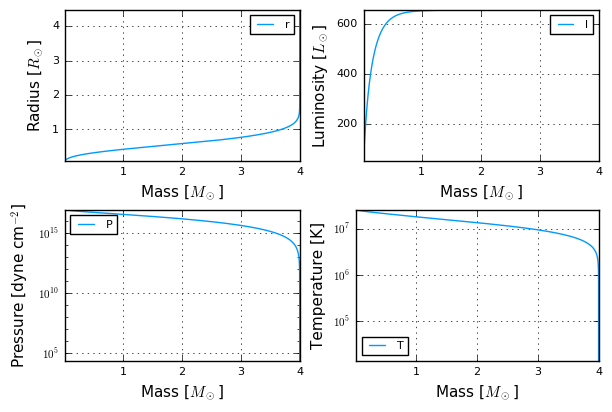
\includegraphics[width=0.9\linewidth]{mstar4.png}
  \caption{Structure profiles for 4 $M_\odot$ solar metallicity test case.}
\end{figure}

\section{Discussion}

The test case runs in less than two minutes on an Intel 2.6 GHz CPU, with a memory usage of 1.24 Gb.  This is a significant advantage compared to other stellar structure codes written in python, for which each iteration of the Newton-Raphson steps could take around a minute.  The code could be significantly sped up by parallelizing the set of integrations for each computation of the Jacobian, and it is clear that the code would benefit from a more careful treatment of space utilization.

Julia is a different beast than python.  While there are a number of third party numeric libraries out there already for Julia, the community has not yet converged on a unified scientific stack in the same way that python has unified behind numpy and scipy.  I ended up implementing my own Runge-Kutta integrator and my own Newton-Raphson zero finding code, almost directly out of Numerical Recipes, which served my purposes well enough.  Having come from a background in mostly python, learning Julia brought a number of challenges, from relatively minor ones like its one-based array indexing, to trickier ones like the shift from object-oriented programming to a more functional programming style.  My personal verdict is that Julia shows much promise for developing tools to tackle numerically challenging problems, but it is not going to replace python as my general purpose scripting language anytime in the near future.

\end{document}

%%% Local Variables:
%%% mode: latex
%%% TeX-master: t
%%% End:
